% if you have a percent symbol, that line is commenting like in programming languages. it does not do anything.

% here, i specify the general style of the document. 
% you can play with it to see what changes, for example try removing twocolumn
\documentclass[aps,twocolumn,showpacs,preprintnumbers,nofootinbib,prl,superscriptaddress,groupedaddress]{revtex4-2}

% here are some "packages", basically utilities i need in this document. not all documents need all
% packages
\usepackage{amssymb,graphicx}
\usepackage{amsmath}
\usepackage{multirow}
\usepackage{epsfig}
\usepackage[usenames]{color} 
\usepackage[export]{adjustbox}
\usepackage{mathtools}
\usepackage{hyperref}
\usepackage{enumitem}
\usepackage{graphicx}

% you can define your own shortcuts etc, if you use sth very often
\newcommand{\balign}{\begin{align}}
\newcommand{\ealign}{\end{align}}

% or you can define your own symbols, check what this is
\def\meff{m_{\textrm{eff}}}


% here is where the document begins
\begin{document}

\title{PHYS414/514 Final Project}
\author{Baran Berkay H\"okelek} % turkish characters require special handling
\affiliation{Department of Physics, Ko\c{c} University, \\
Rumelifeneri Yolu, 34450 Sariyer, Istanbul, Turkey }
\date{\today}

\begin{abstract}
In this project, the structures of various stars are calculated with Newtonian Mechanics, General Relativity(GR) and alternate theories of gravity. This document contains the derivation and discussion of the actual physical \& mathematical results, and also the details of the coding; such as unit testing and convergence. 
\end{abstract}
\maketitle


%%%%%%%%%%%%%%%%%%%%%%%%%%%%%%%%%%%%%%%%
\section{Newton}
%%%%%%%%%%%%%%%%%%%%%%%%%%%%%%%%%%%%%%%%
%%%%%%%%%%%%%%%%%%%%%%%%%%%%%%%%%%%%%%%%
\begin{enumerate}[label=(\alph*)]
    \item We know that \\
    \begin{align}
        \frac{dm(r)}{dr} = 4\pi r^{2}\rho(r)\label{dmass}    \\
        \frac{dp(r)}{dr} = -\frac{Gm(r)\rho(r)}{r^{2}}\label{dpress}  \\
        p(r) = K{\rho(r)}^{1+\frac{1}{n}}\label{press} 
    \end{align}
    \eqref{dpress} can be rewritten as:
    \begin{equation}
      \frac{1}{\rho}\frac{dp}{dr} = -\frac{Gm}{r^{2}}
    \end{equation}
    whose derivative with respect to $r$ yields
    \begin{align}
        \frac{d}{dr}\left(\frac{1}{\rho}\frac{dp}{dr}\right) = \frac{2Gm}{r^{3}} - \frac{G}{r^{2}}\frac{dm}{dr}    \nonumber \\
        =-\frac{2}{r}\left(\frac{1}{\rho}\frac{dp}{dr}\right) - 4\pi G\rho \label{1/rhodpress}
    \end{align}
    By multiplying Eq.\eqref{1/rhodpress} with $r^{2}$, and collecting the $r$ derivatives of $p$ on one side, we get:
    \begin{align}
        \frac{d}{dr}\left(\frac{r^{2}}{\rho}\frac{dp}{dr}\right) = -4\pi Gr^{2}\rho \label{2nddevrho}
    \end{align}
    Now, we will apply the first portion of the scaling of variables. By introducing a new function $\theta$, which satisfies the relation $\rho = \rho_{c}\theta^{n}$($\rho_{c}$ is a constant), we can rewrite Eq.\eqref{press} as:
    \begin{equation}
        p = K  \rho_{c}^{1+\frac{1}{n}}\theta^{n+1} \label{newpress}
    \end{equation}
    Inserting Eq.\eqref{newpress} into \eqref{2nddevrho}, we get:
    \begin{equation}
        \frac{d}{dr}\left(\frac{r^{2}}{\rho_{c}\theta^{n}}K\rho_{c}^{\frac{1}{n} + 1}(n+1)\theta^{n} \frac{d\theta}{dr}\right) = -4G\pi r^{2}\rho_{c}\theta^{n}
    \end{equation}
    which simplifies to
    \begin{equation}
        \frac{1}{r^{2}}\frac{d}{dr}\left(r^{2}K\rho_{c}^{\frac{1-n}{n}}(n+1)\frac{d\theta}{dr}\right) = -4G\pi \rho_{c}\theta^{n} \label{lastbeforefinal}
    \end{equation}
    Now, here comes the second part of the scaling of variables. By defining $\alpha \coloneqq \sqrt{K\rho_{c}^{\frac{1-n}{n}}(n+1)/4\pi G}$ and introducing a new variable $\xi$ which satisfies the relation $r = \alpha\xi$, we can rewrite Eq.\eqref{lastbeforefinal} as:
    \begin{equation}
        \frac{1}{\xi^{2}}\frac{d}{d\xi} \left(\xi^{2}\frac{d\theta}{d\xi}\right) + \theta^{n} = 0 \label{laneemden}
    \end{equation}
    which is the Lane-Emden equation.
    
    Analytical solutions of Lane-Emden equation only exist for $n=0,1,5$. The regular solutions near the center($\xi\approx 0$) can be approximated as a power series:
    \begin{equation}
        \theta(\xi) = 1 - \frac{1}{6}\xi^{2} + \frac{n}{120}\xi^{4} + \dots
    \end{equation}
    This series has an error of order $O(\xi^{6})$.
    
    The Mathematica code used to calculate this series expression can be found in the Supplementary Material.
    
    Eq.\eqref{dmass} can be rewritten as
    \begin{equation}
        dm(r) = 4\pi r^{2}\rho(r)dr \label{dmassnew}
    \end{equation}
    which, after scaling the appropriate variables ($\rho = \rho_{c}$ , $r = \alpha\xi$), becomes
    \begin{equation}
        dm = 4\pi \rho_{c} \alpha^{3}\xi^{2} \theta^{n}d\xi 
    \end{equation}
    Integrating both sides from $0$ to $\xi_{n}$ gives
    \begin{align}
        m = 4\pi \rho_{c} \alpha^{3} \int_{0}^{\xi_{n}} \xi^{2} \theta^{n}d\xi \nonumber \\
          = 4\pi \rho_{c} \alpha^{3} \int_{0}^{\xi_{n}} -\frac{d}{d\xi} \left(\xi^{2}\frac{d\theta}{d\xi}\right) d\xi \nonumber \\
        = 4\pi \rho_{c} \alpha^{3}\xi_{n}^{2} \left(-\theta '(\xi_{n}) \right) \label{mass}
    \end{align}
    Since $r = \alpha\xi$ and $\xi_{n}$ is the maximum value of $\xi$ where $\theta(\xi) \geq 0$, we can conclude that $R = \alpha\xi_{n}$ is the radius of the star. Multiplying and dividing Eq.\eqref{mass} with $\xi_{n}$ to write it in terms of $R$, we get:
    \begin{equation}
        M = 4\pi \rho_{c} R^{3} \left(-\frac{\theta '(\xi_{n})}{\xi_{n}} \right)
    \end{equation}
    In order to find the total mass of a star in terms of its radius, we need to combine Eq.\eqref{mass} and the fact that $R = \alpha\xi_{n}$.
    
    We'll get rid of $\alpha$, and write its true value instead, with the aim to connect the two equations by isolating $\rho_{c}$ in each one. Eq.\eqref{mass}, with this prescription, can be written as:
    \begin{equation}
        M = 4\pi \left(\frac{K(n+1)}{4\pi G}\right)^{\frac{3}{2}} \left(-\xi_{n}^{2}\theta '(\xi_{n})\right) \rho_{c}^{\frac{3-n}{2n}}
    \end{equation}
    Similarly, 
    \begin{equation}
        R = \alpha\xi_{n} = \left(\frac{K(n+1)}{4\pi G}\right)^{\frac{1}{2}} \xi_{n} \rho_{c}^{\frac{1-n}{2n}}
    \end{equation}
    Isolating $\rho_{c}$ form both equations, we get:
    \begin{align}
        \rho_{c} = \left( \frac{M}{4\pi \left(\frac{K(n+1)}{4\pi G}\right)^{\frac{3}{2}} \left(-\xi_{n}^{2}\theta '(\xi_{n})\right)} \right)^{\frac{2n}{3-n}}     \nonumber \\
        = \left( \frac{R}{\left(\frac{K(n+1)}{4\pi G}\right)^{\frac{1}{2}} \xi_{n}} \right)^{\frac{2n}{1-n}}
    \end{align}
    which results in the relation:
    \begin{equation}
        M = 4\pi \left(\frac{K(n+1)}{G}\right)^{-n} \xi_{n}^{-(1+n)} {\theta '(\xi_{n})}^{1-n} R^{\frac{3-n}{1-n}}
    \end{equation}
    \item The Phython code for extracting the $.csv$ file can be found in the Supplementary Material. The $M$ vs $R$ plot of the white dwarfs is included in Figure 1.
    \begin{figure}[h] 
    \centering
    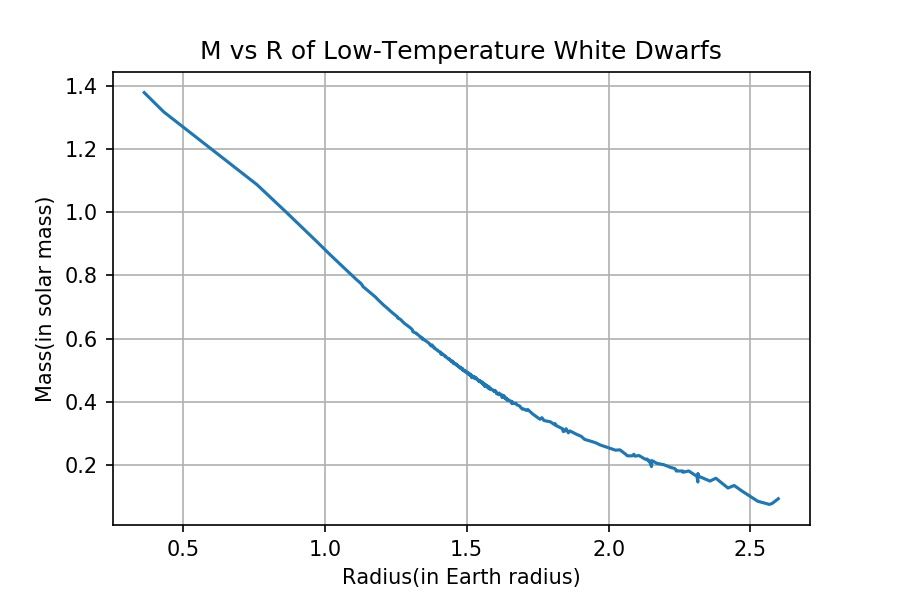
\includegraphics[width=0.5\textwidth]{WDMR.jpg}
    \caption{M-R plot of low-temperature white dwarfs.}
    \end{figure}
    
\end{enumerate}
\end{document}
